Рассмотрим первый пример.

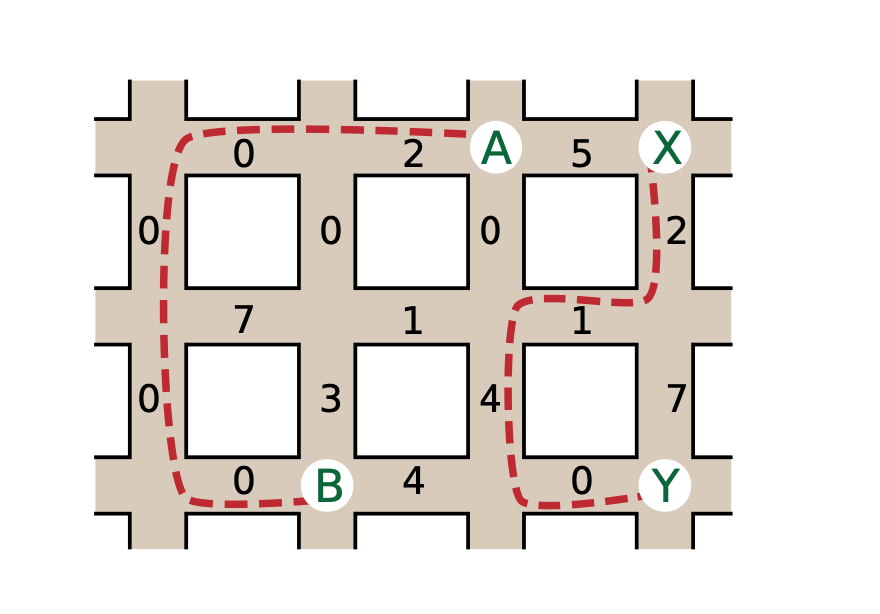
\includegraphics{wombats2.png}

Рисунок выше описывает начальную дорожную решетку, состоящую из $R = 3$ горизонтальных дорог и $C = 4$ вертикальных дорог, для каждого участка дороги указано изначальное количество вомбатов. Рассмотрим следующую последовательность событий:
\begin{itemize}
\item Человек появляется на перекрестке $A = (0,2)$ и собирается спастись на перекрестке $B = (2,1)$. Наименьшее число вомбатов, которое он встретит, равно $2$. Оптимальный путь показан на рисунке пунктиром.
\item Еще один человек появляется на перекрестке $X = (0,3)$ и собирается спастись на перекрестке $Y = (2,3)$. Наименьшее число вомбатов, которое ему придется встретить, равно $7$. Оптимальный путь также обозначен пунктиром.
\item Происходят два события ­изменения: количество вомбатов на верхнем участке вертикальной дороги с номером $0$ изменяется и становится равным $5$, и количество вомбатов на среднем участке горизонтальной дороги с номером $1$ изменяется и становится равным $6$. Обратите внимание на рисунок ниже, на нем измененные числа обведены.

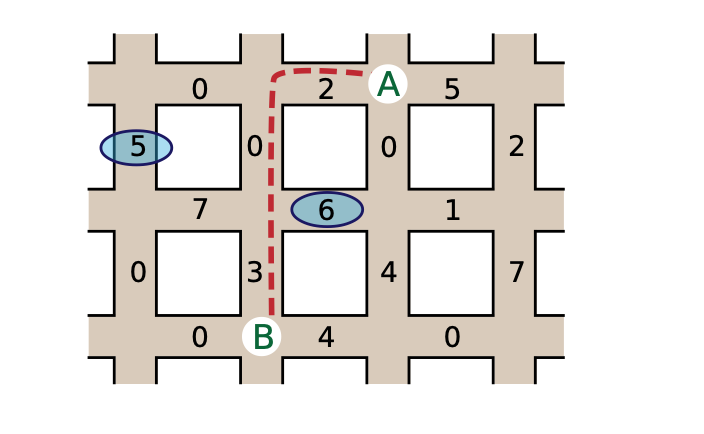
\includegraphics{wombats3.png}

\item Третий человек появляется на перекрестке $A = (0,2)$ и собирается спастись на перекрестке $B = (2,1)$. Теперь наименьшее число вомбатов, которое ему придется встретить на своем пути, равно $5$. Оптимальный путь обозначен пунктиром.
\end{itemize}

Ваше решение должно содержать \t{\#include "wombats.h"}